% ---------------------------------------------------------------------
% The noise model, from zero signal processing.
%
% A self-contained companion to docs/access_tight_rms_bound.tex: only
% the noise side, written for a reader who has not worked with FFTs,
% bands, or filters before.  Every signal-processing idea used by the
% model is built up first, one step at a time, then the model itself
% is assembled from those pieces.
%
% Figures are shared with the main document:
%     python analysis/noise_spectrum_figure.py docs/fig_noise_spectrum.png
%     python analysis/sg_bound_bars.py         docs/fig_sg_bars.png
% ---------------------------------------------------------------------

\documentclass[10pt]{article}
\usepackage[a4paper,margin=22mm]{geometry}
\usepackage{amsmath,amssymb,booktabs,graphicx,array}
\setlength{\parskip}{0.35em}\setlength{\parindent}{0pt}
\newcommand{\rms}{\mathrm{RMS}}
\newcommand{\Mdot}{\dot M}
\title{\vspace{-16mm}\textbf{The noise model, from zero signal
processing}\vspace{-3mm}}
\date{\small companion to \emph{The residual bound, step by step};
equation numbers (19), (19b), (20) refer to that document}
\begin{document}\maketitle

\section{The problem in one sentence}

The residual cap (20) needs one number per run: an upper bound on
$\rms(n)$, the root-mean-square of the disturbance $n$ inside the fit
window. The difficulty is that $n$ is never observed alone --- the
gyro records $y = \text{(smooth rigid-body motion)} + n$, the two are
stuck together in time, and there is no ground-truth curve to
subtract. Everything in this note is one strategy for un-sticking
them: \emph{in time the two are inseparable, but in frequency they
barely overlap.} The model motion is slow; much of the disturbance is
fast. Split the record by frequency and the fast part is pure
disturbance, measured, not assumed; the slow part is then recovered
by a measured ratio. The note first builds the small signal-processing
kit this needs (Sec.~2), then assembles the model (Secs.~3--6), and
closes with why the obvious simpler alternatives fail (Sec.~7) and
what the campaign checks show (Sec.~8). A glossary is at the end.

\section{A five-minute signal-processing kit}

\subsection{A record is a vector}

The window contains $N$ samples $r_1, \dots, r_N$ taken every $T_s$
seconds (here $T_s \approx 5$ ms, $N \approx 80$--$300$, window
length $T = NT_s \approx 0.4$--$0.7$ s). Treat them as one vector
$r \in \mathbb{R}^N$. Its size is measured by the root mean square,
\begin{equation}
  \rms(r) \;=\; \sqrt{\tfrac1N \textstyle\sum_i r_i^2}
  \;=\; \frac{\|r\|}{\sqrt N},
  \tag{N1}
\end{equation}
which is just the vector's Euclidean length, normalised so it does
not grow with $N$. Everything below is linear algebra on this vector;
no probability is needed until the very end.

\subsection{The DFT: the same vector in new coordinates}

The discrete Fourier transform (DFT; the FFT is merely its fast
implementation) does not modify the record. It re-expresses the same
vector in a different orthogonal basis: instead of ``sample 1,
sample 2, \dots'' the coordinates become ``how much of a sinusoid at
frequency $f_k$ is in the record'', for the specific grid of
frequencies
\begin{equation}
  f_k \;=\; \frac{k}{T}, \qquad k = 0, 1, 2, \dots
  \tag{N2}
\end{equation}
Each grid frequency is called a \emph{bin}. Two things about (N2) are
worth pausing on. First, the spacing is $\Delta f = 1/T$: a longer
window gives finer frequency resolution --- our windows give
$\Delta f \approx 1.4$--$2.5$ Hz, so the shortest windows have only
two or three bins below $5$ Hz. Second, $k=0$ is the \emph{DC bin},
the record's mean; we always subtract the mean first, so it plays no
role. For a real-valued record the negative-frequency half of the
transform is the mirror image of the positive half, so one keeps only
$k \ge 0$ (this is the \texttt{rfft}). The largest usable frequency
is the Nyquist frequency $1/(2T_s) \approx 100$ Hz --- faster
oscillations cannot be represented by samples this far apart.

Each bin carries an amplitude: bin $k$'s amplitude is the size of the
sinusoid at $f_k$ contained in the record. A bar chart of amplitude
against $f_k$ is the record's \emph{spectrum} ---
Fig.~\ref{fig:spec}(a) shows the actual bins of one run.

\subsection{Parseval: Pythagoras in disguise}

Because the sinusoids of the DFT are an \emph{orthogonal} basis ---
perpendicular directions in $\mathbb{R}^N$, exactly like rotated
coordinate axes --- the squared length of the vector is the sum of
squared coordinates in either basis:
\begin{equation}
  \textstyle\sum_i r_i^2 \;=\; \text{(sum of squared bin contents)}.
  \tag{N3}
\end{equation}
This is Parseval's identity, and it is nothing deeper than
Pythagoras: energy is counted once per perpendicular direction,
whether the directions are ``samples'' or ``frequencies''. Its
practical meaning: $\rms(r)^2$ can be split \emph{exactly} across
groups of bins.

\subsection{Bands, and the brick-wall split}

A \emph{band} is a set of bins --- ``below $5$ Hz'' (the low band),
``above $5$ Hz'' (the high band). The \emph{brick-wall split} at a
cutoff $f_c$ is the crudest possible filter and, for our purpose, the
best one: transform the record, hand every bin \emph{wholly} to one
side of $f_c$, transform each side back. This produces two time
records $r = r_{\rm lo} + r_{\rm hi}$ that are built from
\emph{disjoint} sets of basis directions, hence exactly orthogonal
($\sum_i r_{{\rm lo},i}\,r_{{\rm hi},i} = 0$), hence
\begin{equation}
  \rms(r)^2 \;=\; \rms(r_{\rm lo})^2 + \rms(r_{\rm hi})^2
  \qquad\text{with no cross term, no approximation.}
  \tag{N4}
\end{equation}
Checked on all $140$ runs, the inner product and the Pythagoras error
are $6\times10^{-16}$ --- machine precision. A ``smoother'' filter (a
Butterworth-shaped mask, the kind used in real-time control loops)
would share the transition-band bins \emph{partially} between the two
sides; the parts are then no longer orthogonal, and on the same data
(N4) acquires a $19\%$ error. The brick wall is what buys the equals
sign, and the equals sign is what the whole construction leans on.

\subsection{Where a smooth curve lives}

The rigid-body motion in the window --- the cosh branch, its error
$e_\omega$, the bias --- evolves on the pendulum timescale: its
spectral home is $C_2/2\pi \approx 0.6$--$0.9$ Hz, and being a smooth
exponential-type curve its bin amplitudes fall away steeply above a
few hertz. Above $5$ Hz the model family can produce \emph{nothing}:
whatever the record contains there is disturbance, by construction
rather than by assumption. This single fact is the foundation of the
model; Fig.~\ref{fig:spec}(b) shows it directly --- the fitted branch
(orange) collapses above a few hertz while the record (blue) does
not.

\subsection{Leakage: the finite-window trap}

One honest complication. The DFT silently treats the $N$ samples as
one period of a repeating signal. A record that ends at a different
level than it began (ours rise monotonically) therefore contains an
artificial jump at the seam, and a jump excites \emph{every} bin ---
this is \emph{(truncation) leakage}, and it is why the high band of
the \emph{raw} record is useless: the leaked tail of the smooth
branch is $4$--$14\times$ the disturbance up there. There are two
standard cures, and the model uses both in different places:
\begin{itemize}
  \setlength\itemsep{0.1em}
  \item \emph{Subtract before splitting.} If a curve carrying the
  same trend is subtracted first, its leakage is subtracted too; the
  remainder is nearly seam-free and its high band is clean. This is
  what both the residual anchor (Sec.~3) and the Savitzky--Golay
  anchor (Sec.~5) do --- they differ only in \emph{which} curve is
  subtracted.
  \item \emph{Taper for display.} Multiplying the record by a window
  that fades to zero at both ends (a Hann taper) removes the seam and
  gives readable spectra. The display panels of
  Fig.~\ref{fig:spec}(b) are tapered; the \emph{numbers} never are
  --- they come from the raw bins of panel (a), where subtraction has
  already cancelled the leakage.
\end{itemize}

\subsection{Quadrature addition, and the shape ratio}

Rearranging (N4): if the low/high ratio
$\kappa = \rms(r_{\rm lo})/\rms(r_{\rm hi})$ is known, the total
follows from the high band alone,
\begin{equation}
  \rms(r) \;=\; \rms(r_{\rm hi})\sqrt{1 + \kappa^2}.
  \tag{N5}
\end{equation}
Orthogonal parts add like perpendicular legs of a triangle
(``in quadrature''), never linearly. The factor $\sqrt{1+\kappa^2}$
converts a \emph{level} (how big the high band is) using a
\emph{shape} (how the energy is distributed across frequency). The
entire noise model is (N5) applied to the disturbance: measure the
level where the model cannot reach, supply the shape from
measurements the model cannot influence.

\begin{figure}[t]
\centering
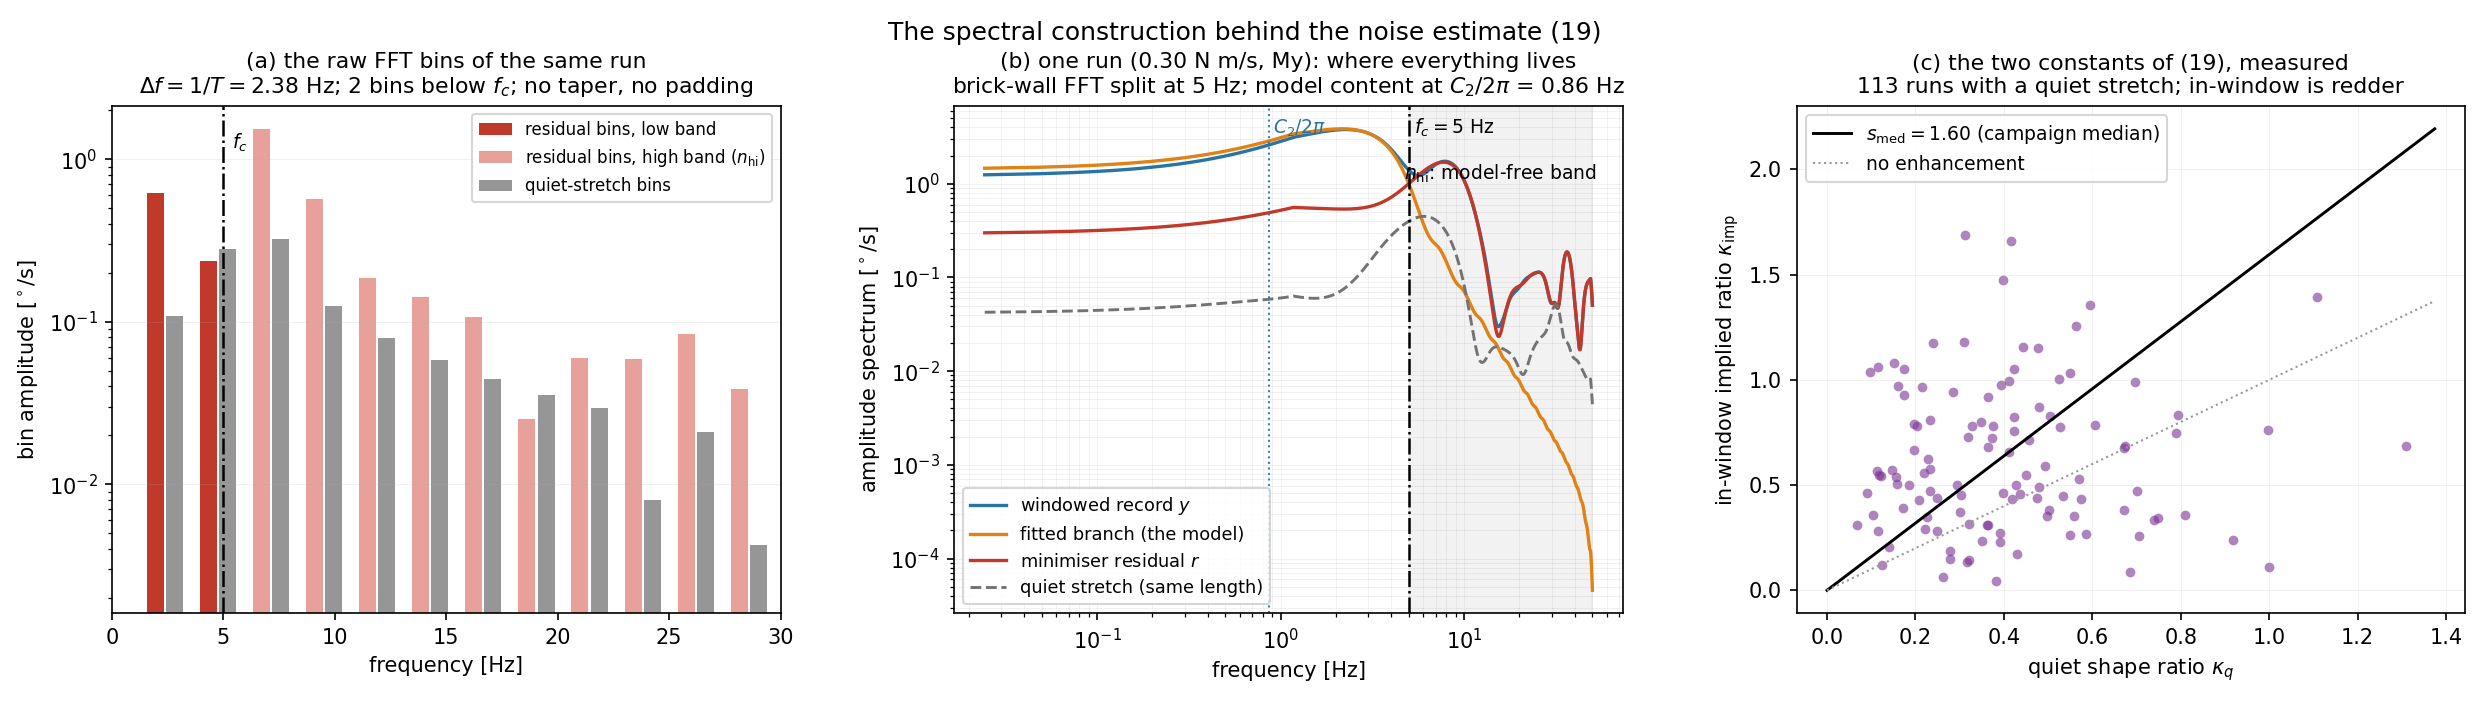
\includegraphics[width=\linewidth]{fig_noise_spectrum.png}
\caption{The construction, drawn. \emph{(a)} The raw FFT bins of one
run's residual and quiet stretch --- one bar per bin $f_k = k/T$,
split at $f_c = 5$ Hz, no taper: these are the exact objects every
number below sums over. \emph{(b)} Smoothed display spectra of the
same run: the record (blue), the fitted branch (orange) collapsing
above a few hertz, the residual (red) riding the record in the high
band, the quiet stretch (grey) below it. \emph{(c)} The two measured
ratios across the campaign: quiet shape $\kappa_q$ against in-window
implied $\kappa_{\rm imp}$; the line is the median enhancement
$s_{\rm med} = 1.60$.}
\label{fig:spec}
\end{figure}

\section{The anchor: the high band of the residual}

The \emph{minimiser residual} $r = y - \hat\omega$ (record minus
fitted branch) has had the trend subtracted, so its high band is
leakage-free; and above $5$ Hz the subtracted branch changed nothing,
since the model has nothing there. Hence
\begin{equation}
  n_{\rm hi} \;\equiv\; r_{\rm hi} \;=\; y_{\rm hi},
  \qquad \rms(n_{\rm hi}) \;=\; \text{the in-window disturbance
  level, measured}.
  \tag{N6}
\end{equation}
$\rms(n_{\rm hi})$ is the one number taken from the run on trust ---
no reference curve, no probability model; the separation is by
frequency alone. One subtlety must be stated precisely: the anchor is
not \emph{fit-free} (subtracting \emph{some} smooth curve was
necessary, Sec.~2.6), but it is \emph{fit-robust} --- swapping the
deployed fit for an entirely different member of the family changes
$\rms(n_{\rm hi})$ by $1.4\%$ at the campaign median. The high band
does not care which good smooth curve was removed; it only needed the
seam gone.

\section{From the high band to the full band: two measured ratios}

(N5) now needs the disturbance's shape ratio $\kappa$. Two
measurements deliver it, from opposite directions.

\emph{The quiet ratio $\kappa_q$.} Before the excitation the vehicle
sits on its gear with rotors at idle: no model motion at all, so a
stretch of that record --- cut to the \emph{same length} as the
window and split by the \emph{same} brick wall --- gives the
disturbance's own low/high ratio with nothing to subtract. Campaign
median $\kappa_q \approx 0.37$: quiet-time disturbance is mostly
high-frequency.

\emph{The implied ratio $\kappa_{\rm imp}$.} The window itself also
implies a ratio, by inverting Pythagoras: (N4) gives
$\rms(r_{\rm lo}) = \sqrt{\rms(r)^2 - \rms(n_{\rm hi})^2}$, both
quantities already in hand, so
\begin{equation}
  \kappa_{\rm imp}
  \;=\; \frac{\sqrt{\rms(r)^2 - \rms(n_{\rm hi})^2}}{\rms(n_{\rm hi})}.
  \tag{N7}
\end{equation}
Its low band contains any unabsorbed model remainder as well, so
$\kappa_{\rm imp}$ errs \emph{high} --- the safe direction: model
leftovers get charged to the noise term, never hidden.

\emph{The enhancement $s_{\rm med}$.} In the window the vehicle
pivots on a gear edge under a growing moment; that contact pumps the
\emph{low} band, so the in-window disturbance is ``redder'' than
quiet-time disturbance. The campaign median of
$\kappa_{\rm imp}/\kappa_q$ over the $113$ runs with a usable quiet
stretch is $s_{\rm med} = 1.60$
(Fig.~\ref{fig:spec}(c)) --- in-window shape $\approx$ quiet shape
scaled by $1.6$.

\section{The estimate (19), and the Savitzky--Golay anchor}

\emph{The estimate.} Assembling (N5) with the corrected shape gives
the main document's equation (19),
$\hat n = \rms(n_{\rm hi})\sqrt{1+(s_{\rm med}\kappa_q)^2}$ --- the
best available \emph{estimate} of $\rms(n)$, used for interpretation
(e.g.\ Sec.~7 of the main document shows the measured residual sits
statistically at $\hat n$). It is deliberately \emph{not} what the
cap uses: a median-calibrated estimate is exceeded by roughly half
the runs, and its anchor comes from the minimiser residual --- the
very object the cap bounds. A guarantee should touch neither.

\emph{The Savitzky--Golay anchor.} To free the anchor from the fit
entirely, replace the subtracted curve (Sec.~2.6) by a generic
smoother that has never heard of the cosh family. A Savitzky--Golay
(SG) filter slides a short window along the record and replaces each
sample by the value of a least-squares cubic fitted \emph{locally}
inside that window --- a moving polynomial smoother, standard in
chemistry and spectroscopy for a half-century. Its window length sets
what it can follow: choosing $\approx 2/(f_c T_s)$ samples makes it
track everything slower than about $f_c$ and nothing faster, so
(record $-$ SG smooth) carries the disturbance's high band with the
trend --- and its leakage --- removed. The same brick wall then reads
off the level. Per run:
\begin{equation}
  N_{\rm SG} \;=\; \rms\big[(y - \mathrm{SG}(y))_{\rm hi}\big],
  \qquad
  N_{\rm med} \;=\; \mathrm{median}_{\rm campaign}\, N_{\rm SG}
  \;=\; 0.77^\circ/\text{s}.
  \tag{N8}
\end{equation}
Three cross-checks say this number is real, not an artefact of the
smoother: a degree-$4$ Legendre polynomial detrend gives
$1.00\times$ the SG anchor at the campaign median, a DCT-based split
gives $1.23\times$, and the fit-robust residual anchor of (N6) gives
$1.03\times$ --- four independent routes, one level.

\section{The adopted constant: $N_n = 3N_{\rm med}$}

The cap's noise term is one campaign constant, the main document's
(19b):
\begin{equation}
  N_n \;=\; 3\,N_{\rm med} \;=\; 2.31^\circ/\text{s}
  \qquad\text{for every run.}
  \tag{N9}
\end{equation}
The factor $3$ is \emph{declared} --- an engineering safety factor
stated up front, not fitted --- and it is sized by the two distinct
jobs the constant must do at once:
\begin{center}\small
\begin{tabular}{@{}llll@{}}
\toprule
job & factor & measured basis & acts\\
\midrule
shape: high band $\to$ full band, (N5) & $1.96$ &
  $\sqrt{1+\kappa^2}$ at the largest ratio $1.69$ & within-run\\
level: median anchor $\to$ every run & $1.5$ &
  anchor max/median $= 2.35$ & between-run\\
\bottomrule
\end{tabular}
\end{center}
$1.96 \times 1.5 = 2.94$, rounded up to $3$. The two halves cannot
absorb each other: no shape factor, however large, covers a run whose
\emph{level} is twice the median. Empirically the minimum total
factor that covers the campaign is $2.05$, and the shape ceiling
alone ($1.96$) leaves exactly the two level-outlier runs outside ---
the declared $3$ carries $46\%$ headroom over the minimum. The
statement is falsifiable in advance: the noise term fails only if a
future run's disturbance exceeds three times the campaign-median
anchor. Fig.~\ref{fig:bars} shows the result: one grey block of
identical height on every bar, no model curve, no minimiser, no
per-run tuning anywhere in the noise side.

\begin{figure}[t]
\centering
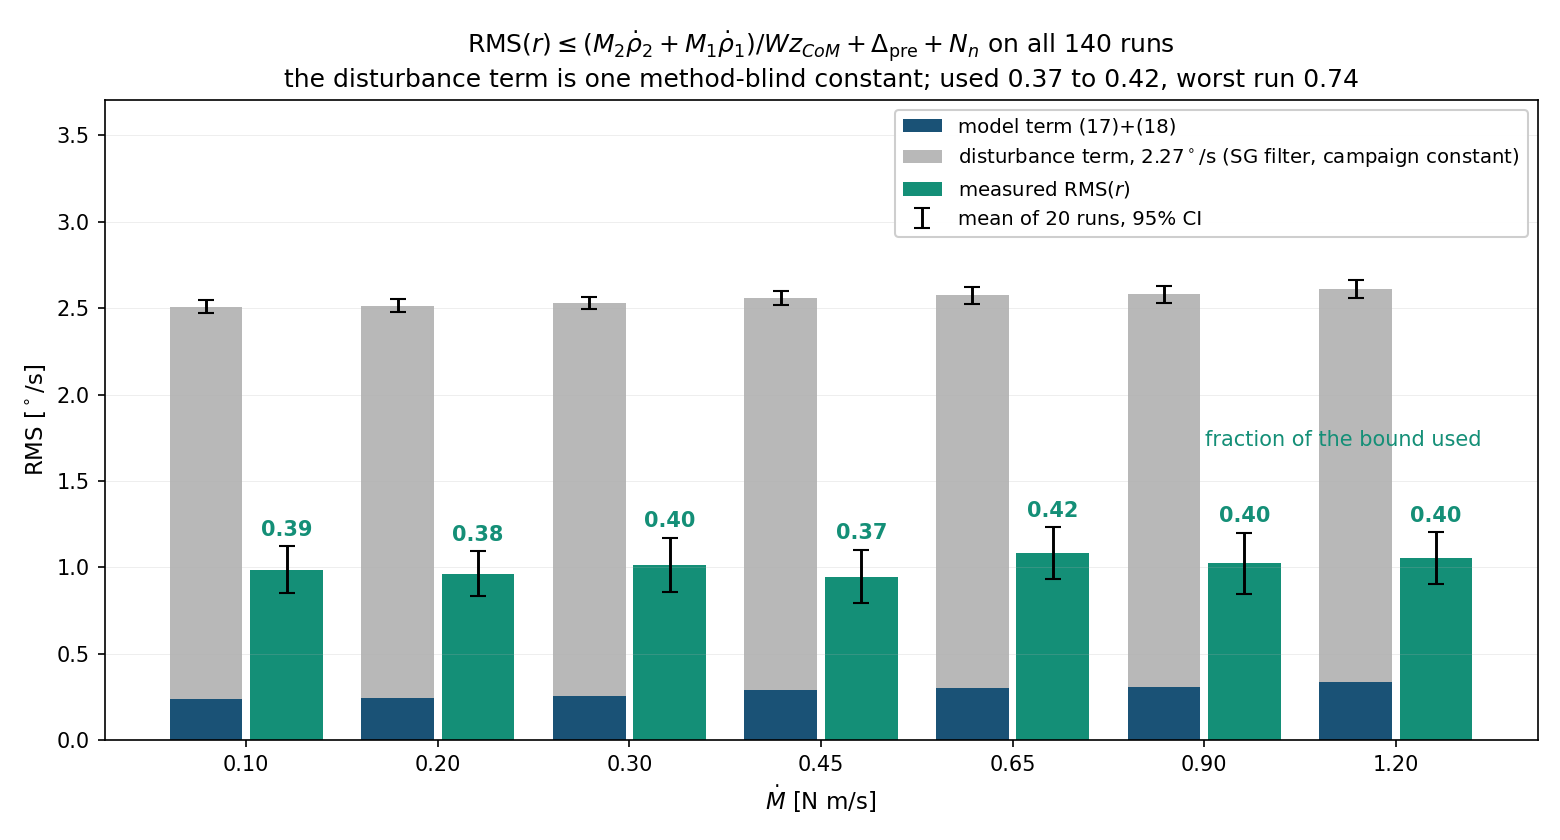
\includegraphics[width=0.9\linewidth]{fig_sg_bars.png}
\caption{The cap (20) with the constant noise term (N9) against the
campaign: model term (dark blue) $+$ $N_n$ (grey) versus the measured
residual (green), means over $20$ runs per rate with $95\%$
intervals. All $140$ runs inside; used fraction $0.36$--$0.41$, worst
run $0.72$.}
\label{fig:bars}
\end{figure}

\section{Why not the obvious simpler things}

Each rejected alternative fails for a reason worth knowing, because
each failure motivates one design choice above.

\emph{``Use the pre-onset noise floor times $k$.''} The quiet gyro
floor is $\approx 0.17^\circ$/s RMS --- but the in-window disturbance
is \emph{contact-borne} (pivoting on a gear edge, motor load rising),
not sensor noise, and runs $2$ to $50\times$ that floor, with no
usable quiet stretch at all on $25$ of $140$ runs. One constant $k$
covering the spread would be $k = 49$, collapsing the cap's used
fraction to $0.16$. \emph{Lesson: the level must be measured in the
window itself} --- which is what (N6) and (N8) do.

\emph{``Use a textbook noise estimator.''} The two standard fit-free
estimators --- the second-difference formula and the finest-scale
wavelet MAD --- read $0.47\times$ and $0.65\times$ the true high-band
level here. Both anchor at the very top of the band (near Nyquist),
and this disturbance is \emph{coloured} --- its spectrum falls with
frequency --- so the top of the band is its quietest corner; the MAD
variant additionally discounts bursts. Swapped into the cap they fail
$59/140$ and $13/140$ runs. \emph{Lesson: integrate the whole
model-free band, not its quietest corner.}

\emph{``Split the raw record; skip the subtraction.''} Truncation
leakage (Sec.~2.6) makes the raw high band read $4$--$14\times$ too
high. \emph{Lesson: subtract a trend first; any good one works.}

\emph{``Keep the per-run envelope.''} The per-run form
$\rms(n_{\rm hi})\sqrt{1+\kappa_{\sup}^2}$ is tighter (mean used
$\approx 0.50$) but its anchor comes from the minimiser residual ---
defensible (it is fit-robust), yet a reader can still object that the
method's own output appears in the method's own guarantee. The
constant (N9) removes the objection at a known price.

\emph{``Take the campaign maximum; declare nothing.''} The maximum SG
anchor with the shape ceiling gives $3.6^\circ$/s --- every
multiplier an observed extreme, no judgment anywhere --- at mean used
$0.26$. Valid, and the natural endpoint for a maximally sceptical
reader; (N9) sits one step tighter with one declared number.

\section{What the checks show}

On the $140$-run campaign, with the model term of the main document:
the cap holds on $140/140$ runs; the used fraction is
$0.36$--$0.41$ by rate (per-run: p10 $0.24$, median $0.38$, worst
$0.72$); the split's orthogonality is machine-exact ($6\times
10^{-16}$); moving the cutoff to $2$ or $3$ Hz changes nothing
($140/140$ either way) because a total does not depend on where it is
split --- only past $8$ Hz, where too few bins remain above the
cutoff, does the construction degrade; and the anchor is insensitive
to the subtracted curve at the $1.4\%$ level. The residual itself
sits at the noise estimate ($\rms(r)/\hat n$: median $0.976$, IQR
$0.89$--$1.09$, flat across a twelvefold rate change) --- the
disturbance floor is what the fit leaves behind, and the model error
underneath it ($0.16$--$0.17^\circ$/s) is invisible at this floor,
exactly as the theory predicts.

\section*{Glossary}

\begin{center}\small
\begin{tabular}{@{}lp{0.78\linewidth}@{}}
\toprule
bin & one frequency $f_k = k/T$ of the DFT grid; the record's
      content at that frequency\\
$\Delta f$ & bin spacing $= 1/T$; longer window $\Rightarrow$ finer
      frequency grid\\
DC bin & the $k=0$ bin $=$ the record's mean; removed before
      everything\\
Nyquist & the fastest representable frequency, $1/(2T_s)$\\
spectrum & bin amplitude drawn against frequency\\
band & a set of bins (``below $5$ Hz'', ``above $5$ Hz'')\\
brick-wall split & every bin handed wholly to one band; makes the two
      parts exactly orthogonal\\
orthogonal & perpendicular as vectors: $\sum_i a_ib_i = 0$; sizes
      then add by Pythagoras\\
Parseval & Pythagoras across the DFT basis: total energy $=$ sum of
      bin energies\\
quadrature & adding orthogonal parts as $\sqrt{a^2+b^2}$, never
      $a+b$\\
leakage & spill-over of a trend into all bins, caused by the
      finite window's artificial seam\\
taper (Hann) & fading the record to zero at both ends to remove the
      seam; display only here\\
coloured noise & noise whose spectrum is not flat (here: falling
      with frequency)\\
SG filter & Savitzky--Golay: a sliding local least-squares
      polynomial smoother; a generic lowpass\\
quiet stretch & pre-excitation segment, rotors at idle: disturbance
      with no model motion in it\\
$\kappa$ & a low-band/high-band RMS ratio: the \emph{shape} of a
      spectrum in one number\\
anchor & the measured high-band level everything else scales
      from\\
\bottomrule
\end{tabular}
\end{center}

\end{document}
